% Options for packages loaded elsewhere
\PassOptionsToPackage{unicode}{hyperref}
\PassOptionsToPackage{hyphens}{url}
%
\documentclass[
]{article}
\usepackage{amsmath,amssymb}
\usepackage{iftex}
\ifPDFTeX
  \usepackage[T1]{fontenc}
  \usepackage[utf8]{inputenc}
  \usepackage{textcomp} % provide euro and other symbols
\else % if luatex or xetex
  \usepackage{unicode-math} % this also loads fontspec
  \defaultfontfeatures{Scale=MatchLowercase}
  \defaultfontfeatures[\rmfamily]{Ligatures=TeX,Scale=1}
\fi
\usepackage{lmodern}
\ifPDFTeX\else
  % xetex/luatex font selection
\fi
% Use upquote if available, for straight quotes in verbatim environments
\IfFileExists{upquote.sty}{\usepackage{upquote}}{}
\IfFileExists{microtype.sty}{% use microtype if available
  \usepackage[]{microtype}
  \UseMicrotypeSet[protrusion]{basicmath} % disable protrusion for tt fonts
}{}
\makeatletter
\@ifundefined{KOMAClassName}{% if non-KOMA class
  \IfFileExists{parskip.sty}{%
    \usepackage{parskip}
  }{% else
    \setlength{\parindent}{0pt}
    \setlength{\parskip}{6pt plus 2pt minus 1pt}}
}{% if KOMA class
  \KOMAoptions{parskip=half}}
\makeatother
\usepackage{xcolor}
\usepackage[margin=1in]{geometry}
\usepackage{color}
\usepackage{fancyvrb}
\newcommand{\VerbBar}{|}
\newcommand{\VERB}{\Verb[commandchars=\\\{\}]}
\DefineVerbatimEnvironment{Highlighting}{Verbatim}{commandchars=\\\{\}}
% Add ',fontsize=\small' for more characters per line
\usepackage{framed}
\definecolor{shadecolor}{RGB}{248,248,248}
\newenvironment{Shaded}{\begin{snugshade}}{\end{snugshade}}
\newcommand{\AlertTok}[1]{\textcolor[rgb]{0.94,0.16,0.16}{#1}}
\newcommand{\AnnotationTok}[1]{\textcolor[rgb]{0.56,0.35,0.01}{\textbf{\textit{#1}}}}
\newcommand{\AttributeTok}[1]{\textcolor[rgb]{0.13,0.29,0.53}{#1}}
\newcommand{\BaseNTok}[1]{\textcolor[rgb]{0.00,0.00,0.81}{#1}}
\newcommand{\BuiltInTok}[1]{#1}
\newcommand{\CharTok}[1]{\textcolor[rgb]{0.31,0.60,0.02}{#1}}
\newcommand{\CommentTok}[1]{\textcolor[rgb]{0.56,0.35,0.01}{\textit{#1}}}
\newcommand{\CommentVarTok}[1]{\textcolor[rgb]{0.56,0.35,0.01}{\textbf{\textit{#1}}}}
\newcommand{\ConstantTok}[1]{\textcolor[rgb]{0.56,0.35,0.01}{#1}}
\newcommand{\ControlFlowTok}[1]{\textcolor[rgb]{0.13,0.29,0.53}{\textbf{#1}}}
\newcommand{\DataTypeTok}[1]{\textcolor[rgb]{0.13,0.29,0.53}{#1}}
\newcommand{\DecValTok}[1]{\textcolor[rgb]{0.00,0.00,0.81}{#1}}
\newcommand{\DocumentationTok}[1]{\textcolor[rgb]{0.56,0.35,0.01}{\textbf{\textit{#1}}}}
\newcommand{\ErrorTok}[1]{\textcolor[rgb]{0.64,0.00,0.00}{\textbf{#1}}}
\newcommand{\ExtensionTok}[1]{#1}
\newcommand{\FloatTok}[1]{\textcolor[rgb]{0.00,0.00,0.81}{#1}}
\newcommand{\FunctionTok}[1]{\textcolor[rgb]{0.13,0.29,0.53}{\textbf{#1}}}
\newcommand{\ImportTok}[1]{#1}
\newcommand{\InformationTok}[1]{\textcolor[rgb]{0.56,0.35,0.01}{\textbf{\textit{#1}}}}
\newcommand{\KeywordTok}[1]{\textcolor[rgb]{0.13,0.29,0.53}{\textbf{#1}}}
\newcommand{\NormalTok}[1]{#1}
\newcommand{\OperatorTok}[1]{\textcolor[rgb]{0.81,0.36,0.00}{\textbf{#1}}}
\newcommand{\OtherTok}[1]{\textcolor[rgb]{0.56,0.35,0.01}{#1}}
\newcommand{\PreprocessorTok}[1]{\textcolor[rgb]{0.56,0.35,0.01}{\textit{#1}}}
\newcommand{\RegionMarkerTok}[1]{#1}
\newcommand{\SpecialCharTok}[1]{\textcolor[rgb]{0.81,0.36,0.00}{\textbf{#1}}}
\newcommand{\SpecialStringTok}[1]{\textcolor[rgb]{0.31,0.60,0.02}{#1}}
\newcommand{\StringTok}[1]{\textcolor[rgb]{0.31,0.60,0.02}{#1}}
\newcommand{\VariableTok}[1]{\textcolor[rgb]{0.00,0.00,0.00}{#1}}
\newcommand{\VerbatimStringTok}[1]{\textcolor[rgb]{0.31,0.60,0.02}{#1}}
\newcommand{\WarningTok}[1]{\textcolor[rgb]{0.56,0.35,0.01}{\textbf{\textit{#1}}}}
\usepackage{graphicx}
\makeatletter
\newsavebox\pandoc@box
\newcommand*\pandocbounded[1]{% scales image to fit in text height/width
  \sbox\pandoc@box{#1}%
  \Gscale@div\@tempa{\textheight}{\dimexpr\ht\pandoc@box+\dp\pandoc@box\relax}%
  \Gscale@div\@tempb{\linewidth}{\wd\pandoc@box}%
  \ifdim\@tempb\p@<\@tempa\p@\let\@tempa\@tempb\fi% select the smaller of both
  \ifdim\@tempa\p@<\p@\scalebox{\@tempa}{\usebox\pandoc@box}%
  \else\usebox{\pandoc@box}%
  \fi%
}
% Set default figure placement to htbp
\def\fps@figure{htbp}
\makeatother
\setlength{\emergencystretch}{3em} % prevent overfull lines
\providecommand{\tightlist}{%
  \setlength{\itemsep}{0pt}\setlength{\parskip}{0pt}}
\setcounter{secnumdepth}{-\maxdimen} % remove section numbering
\usepackage{bookmark}
\IfFileExists{xurl.sty}{\usepackage{xurl}}{} % add URL line breaks if available
\urlstyle{same}
\hypersetup{
  pdftitle={WK8},
  hidelinks,
  pdfcreator={LaTeX via pandoc}}

\title{WK8}
\author{}
\date{\vspace{-2.5em}2025-08-21}

\begin{document}
\maketitle

\begin{Shaded}
\begin{Highlighting}[]
\FunctionTok{library}\NormalTok{(tidyverse)}
\end{Highlighting}
\end{Shaded}

\begin{verbatim}
## -- Attaching core tidyverse packages ------------------------ tidyverse 2.0.0 --
## v dplyr     1.1.4     v readr     2.1.5
## v forcats   1.0.0     v stringr   1.5.1
## v ggplot2   3.5.2     v tibble    3.2.1
## v lubridate 1.9.4     v tidyr     1.3.1
## v purrr     1.0.4     
## -- Conflicts ------------------------------------------ tidyverse_conflicts() --
## x dplyr::filter() masks stats::filter()
## x dplyr::lag()    masks stats::lag()
## i Use the conflicted package (<http://conflicted.r-lib.org/>) to force all conflicts to become errors
\end{verbatim}

\begin{Shaded}
\begin{Highlighting}[]
\FunctionTok{library}\NormalTok{(readxl)}
\FunctionTok{library}\NormalTok{(lubridate)}
\FunctionTok{library}\NormalTok{(janitor)}
\end{Highlighting}
\end{Shaded}

\begin{verbatim}
## 
## Attaching package: 'janitor'
## 
## The following objects are masked from 'package:stats':
## 
##     chisq.test, fisher.test
\end{verbatim}

\begin{Shaded}
\begin{Highlighting}[]
\FunctionTok{library}\NormalTok{(purrr)}
\FunctionTok{library}\NormalTok{(readr)}
\FunctionTok{library}\NormalTok{(ggthemes)}
\FunctionTok{library}\NormalTok{(ggeffects)}
\FunctionTok{library}\NormalTok{(lme4)}
\end{Highlighting}
\end{Shaded}

\begin{verbatim}
## Loading required package: Matrix
## 
## Attaching package: 'Matrix'
## 
## The following objects are masked from 'package:tidyr':
## 
##     expand, pack, unpack
\end{verbatim}

\begin{Shaded}
\begin{Highlighting}[]
\FunctionTok{library}\NormalTok{(dplyr)}
\FunctionTok{library}\NormalTok{(ggplot2)}
\CommentTok{\#install.packages("emmeans")}
\FunctionTok{library}\NormalTok{(emmeans)      }
\end{Highlighting}
\end{Shaded}

\begin{verbatim}
## Welcome to emmeans.
## Caution: You lose important information if you filter this package's results.
## See '? untidy'
\end{verbatim}

\begin{Shaded}
\begin{Highlighting}[]
\CommentTok{\#install.packages("broom.mixed")}
\FunctionTok{library}\NormalTok{(broom.mixed)  }
\FunctionTok{library}\NormalTok{(viridis)      }
\end{Highlighting}
\end{Shaded}

\begin{verbatim}
## Loading required package: viridisLite
\end{verbatim}

\begin{Shaded}
\begin{Highlighting}[]
\FunctionTok{library}\NormalTok{(nlme)         }
\end{Highlighting}
\end{Shaded}

\begin{verbatim}
## 
## Attaching package: 'nlme'
## 
## The following object is masked from 'package:lme4':
## 
##     lmList
## 
## The following object is masked from 'package:dplyr':
## 
##     collapse
\end{verbatim}

\begin{Shaded}
\begin{Highlighting}[]
\FunctionTok{library}\NormalTok{(mgcv)         }
\end{Highlighting}
\end{Shaded}

\begin{verbatim}
## This is mgcv 1.9-3. For overview type 'help("mgcv-package")'.
\end{verbatim}

\begin{Shaded}
\begin{Highlighting}[]
\CommentTok{\#setwd("C:/Users/Tobyz/Desktop/S.tort{-}light{-}growth/Data")}
\end{Highlighting}
\end{Shaded}

\emph{import plant data}

\begin{Shaded}
\begin{Highlighting}[]
\NormalTok{plant }\OtherTok{\textless{}{-}} \FunctionTok{read.csv}\NormalTok{(}\StringTok{"Data/WL2{-}2023\_Size\_Combined.csv"}\NormalTok{) }\SpecialCharTok{\%\textgreater{}\%}
  \FunctionTok{clean\_names}\NormalTok{() }\SpecialCharTok{\%\textgreater{}\%}
  \FunctionTok{mutate}\NormalTok{(}\AttributeTok{survey\_date =} \FunctionTok{as.Date}\NormalTok{(survey\_date, }\AttributeTok{format =} \StringTok{"\%m/\%d/\%Y"}\NormalTok{))}
\FunctionTok{summary}\NormalTok{(plant)}
\end{Highlighting}
\end{Shaded}

\begin{verbatim}
##   survey_date            block             genotype            pop_mf         
##  Min.   :2023-07-03   Length:17336       Length:17336       Length:17336      
##  1st Qu.:2023-08-02   Class :character   Class :character   Class :character  
##  Median :2023-08-30   Mode  :character   Mode  :character   Mode  :character  
##  Mean   :2023-08-28                                                           
##  3rd Qu.:2023-09-20                                                           
##  Max.   :2023-10-20                                                           
##                                                                               
##   parent_pop              mf              rep           height_cm     
##  Length:17336       Min.   : 1.000   Min.   : 1.000   Min.   : 0.100  
##  Class :character   1st Qu.: 2.000   1st Qu.: 4.000   1st Qu.: 1.700  
##  Mode  :character   Median : 5.000   Median : 8.000   Median : 3.100  
##                     Mean   : 4.584   Mean   : 7.932   Mean   : 4.491  
##                     3rd Qu.: 6.000   3rd Qu.:11.000   3rd Qu.: 5.700  
##                     Max.   :14.000   Max.   :27.000   Max.   :39.400  
##                                                       NA's   :8762    
##   long_leaf_cm   survey_notes      
##  Min.   :0.100   Length:17336      
##  1st Qu.:1.600   Class :character  
##  Median :2.500   Mode  :character  
##  Mean   :2.599                     
##  3rd Qu.:3.500                     
##  Max.   :9.000                     
##  NA's   :9350
\end{verbatim}

\emph{consolidate light measurement to a weekly measurement}

\begin{Shaded}
\begin{Highlighting}[]
\CommentTok{\#import light data}
\NormalTok{light\_raw }\OtherTok{\textless{}{-}} \FunctionTok{read\_csv}\NormalTok{(}\StringTok{"Data/IntBioHalfHourTable\_clean.txt"}\NormalTok{)}
\end{Highlighting}
\end{Shaded}

\begin{verbatim}
## Rows: 4063 Columns: 139
## -- Column specification --------------------------------------------------------
## Delimiter: ","
## dbl  (138): RECORD, BattV_Max, PTemp_C_Max, SlrW_Avg, SlrW_Max, SlrW_Min, Sl...
## dttm   (1): TIMESTAMP
## 
## i Use `spec()` to retrieve the full column specification for this data.
## i Specify the column types or set `show_col_types = FALSE` to quiet this message.
\end{verbatim}

\begin{Shaded}
\begin{Highlighting}[]
\CommentTok{\#weekly measurement}
\NormalTok{weekly\_light }\OtherTok{\textless{}{-}}\NormalTok{ light\_raw }\SpecialCharTok{\%\textgreater{}\%}
  \FunctionTok{mutate}\NormalTok{(}
    \AttributeTok{timestamp =} \FunctionTok{ymd\_hms}\NormalTok{(TIMESTAMP),}
    \AttributeTok{SlrW\_Avg =} \FunctionTok{as.numeric}\NormalTok{(SlrW\_Avg),  }\CommentTok{\# turn into number format}
    \AttributeTok{week =} \FunctionTok{floor\_date}\NormalTok{(timestamp, }\StringTok{"week"}\NormalTok{)}
\NormalTok{  ) }\SpecialCharTok{\%\textgreater{}\%}
  \FunctionTok{group\_by}\NormalTok{(week) }\SpecialCharTok{\%\textgreater{}\%}
  \FunctionTok{summarise}\NormalTok{(}
    \AttributeTok{weekly\_avg\_SlrW =} \FunctionTok{mean}\NormalTok{(SlrW\_Avg, }\AttributeTok{na.rm =} \ConstantTok{TRUE}\NormalTok{),}
    \AttributeTok{.groups =} \StringTok{"drop"}
\NormalTok{  )}
\end{Highlighting}
\end{Shaded}

\begin{verbatim}
## Warning: There was 1 warning in `mutate()`.
## i In argument: `timestamp = ymd_hms(TIMESTAMP)`.
## Caused by warning:
## !  84 failed to parse.
\end{verbatim}

\begin{Shaded}
\begin{Highlighting}[]
\CommentTok{\# result}
\FunctionTok{print}\NormalTok{(weekly\_light)}
\end{Highlighting}
\end{Shaded}

\begin{verbatim}
## # A tibble: 14 x 2
##    week                weekly_avg_SlrW
##    <dttm>                        <dbl>
##  1 2023-07-30 00:00:00         280.   
##  2 2023-08-06 00:00:00         277.   
##  3 2023-08-13 00:00:00         186.   
##  4 2023-08-20 00:00:00         184.   
##  5 2023-08-27 00:00:00         200.   
##  6 2023-09-03 00:00:00         211.   
##  7 2023-09-10 00:00:00         204.   
##  8 2023-09-17 00:00:00         189.   
##  9 2023-09-24 00:00:00         159.   
## 10 2023-10-01 00:00:00         138.   
## 11 2023-10-08 00:00:00         133.   
## 12 2023-10-15 00:00:00         135.   
## 13 2023-10-22 00:00:00         116.   
## 14 NA                           -0.616
\end{verbatim}

\emph{Investigate or filter out plants that show negative growth} \#Q:
How could we deal with bad observations? \#Solution: find out tolerance
value and then filter out observance data lager than the tolerance value
\#Figure A: Histogram showing the frequency of decreases in plant height
between consecutive surveys. Most negative growth values are close to
zero, likely reflecting measurement noise, while a small number of
extreme decreases (\textless=--5 cm) suggest errors and were removed
from subsequent analyses.

\begin{Shaded}
\begin{Highlighting}[]
\CommentTok{\#PID}
\NormalTok{plant\_growth }\OtherTok{\textless{}{-}}\NormalTok{ plant }\SpecialCharTok{\%\textgreater{}\%}
  \FunctionTok{unite}\NormalTok{(}\StringTok{"PID"}\NormalTok{, genotype}\SpecialCharTok{:}\NormalTok{rep, }\AttributeTok{sep =} \StringTok{"\_"}\NormalTok{, }\AttributeTok{remove =} \ConstantTok{FALSE}\NormalTok{) }\SpecialCharTok{\%\textgreater{}\%}
  \FunctionTok{mutate}\NormalTok{(}\AttributeTok{survey\_date =} \FunctionTok{as.Date}\NormalTok{(survey\_date))}

\CommentTok{\#find out plants with negative growth}
\NormalTok{plant\_growth }\SpecialCharTok{\%\textgreater{}\%}
  \FunctionTok{arrange}\NormalTok{(PID, survey\_date) }\SpecialCharTok{\%\textgreater{}\%}  \CommentTok{\# arrange in time sequence}
  \FunctionTok{group\_by}\NormalTok{(PID) }\SpecialCharTok{\%\textgreater{}\%}
  \FunctionTok{mutate}\NormalTok{(}\AttributeTok{growth =}\NormalTok{ height\_cm }\SpecialCharTok{{-}} \FunctionTok{lag}\NormalTok{(height\_cm)) }\SpecialCharTok{\%\textgreater{}\%}  \CommentTok{\# find out the diff btw nearby dates}
  \FunctionTok{summarise}\NormalTok{(}\AttributeTok{has\_negative\_growth =} \FunctionTok{any}\NormalTok{(growth }\SpecialCharTok{\textless{}} \DecValTok{0}\NormalTok{, }\AttributeTok{na.rm =} \ConstantTok{TRUE}\NormalTok{)) }\SpecialCharTok{\%\textgreater{}\%} 
  \FunctionTok{filter}\NormalTok{(has\_negative\_growth) }\OtherTok{{-}\textgreater{}}\NormalTok{ neg\_growth\_plants}
\NormalTok{neg\_growth\_plants}
\end{Highlighting}
\end{Shaded}

\begin{verbatim}
## # A tibble: 826 x 2
##    PID                  has_negative_growth
##    <chr>                <lgl>              
##  1 BH_1_10_BH_1_BH_1_10 TRUE               
##  2 BH_1_12_BH_1_BH_1_12 TRUE               
##  3 BH_1_13_BH_1_BH_1_13 TRUE               
##  4 BH_1_1_BH_1_BH_1_1   TRUE               
##  5 BH_1_4_BH_1_BH_1_4   TRUE               
##  6 BH_1_7_BH_1_BH_1_7   TRUE               
##  7 BH_2_10_BH_2_BH_2_10 TRUE               
##  8 BH_2_11_BH_2_BH_2_11 TRUE               
##  9 BH_2_12_BH_2_BH_2_12 TRUE               
## 10 BH_2_13_BH_2_BH_2_13 TRUE               
## # i 816 more rows
\end{verbatim}

\begin{Shaded}
\begin{Highlighting}[]
\CommentTok{\#find out tolerance value}
\NormalTok{neg\_growth\_values }\OtherTok{\textless{}{-}}\NormalTok{ plant\_growth }\SpecialCharTok{\%\textgreater{}\%}
  \FunctionTok{arrange}\NormalTok{(PID, survey\_date) }\SpecialCharTok{\%\textgreater{}\%}
  \FunctionTok{group\_by}\NormalTok{(PID) }\SpecialCharTok{\%\textgreater{}\%}
  \FunctionTok{mutate}\NormalTok{(}\AttributeTok{growth =}\NormalTok{ height\_cm }\SpecialCharTok{{-}} \FunctionTok{lag}\NormalTok{(height\_cm)) }\SpecialCharTok{\%\textgreater{}\%}
  \FunctionTok{ungroup}\NormalTok{() }\SpecialCharTok{\%\textgreater{}\%}
  \FunctionTok{filter}\NormalTok{(growth }\SpecialCharTok{\textless{}} \DecValTok{0}\NormalTok{)}

\FunctionTok{ggplot}\NormalTok{(neg\_growth\_values, }\FunctionTok{aes}\NormalTok{(}\AttributeTok{x =}\NormalTok{ growth)) }\SpecialCharTok{+}
  \FunctionTok{geom\_histogram}\NormalTok{(}\AttributeTok{binwidth =} \FloatTok{0.5}\NormalTok{, }\AttributeTok{fill =} \StringTok{"red"}\NormalTok{, }\AttributeTok{color =} \StringTok{"black"}\NormalTok{) }\SpecialCharTok{+}
  \FunctionTok{labs}\NormalTok{(}
    \AttributeTok{title =} \StringTok{"Figure A: Distribution of Negative Growth Values"}\NormalTok{,}
    \AttributeTok{x =} \StringTok{"Height Decrease (cm)"}\NormalTok{,}
    \AttributeTok{y =} \StringTok{"Count"}
\NormalTok{  ) }\SpecialCharTok{+}
  \FunctionTok{theme\_bw}\NormalTok{()}
\end{Highlighting}
\end{Shaded}

\pandocbounded{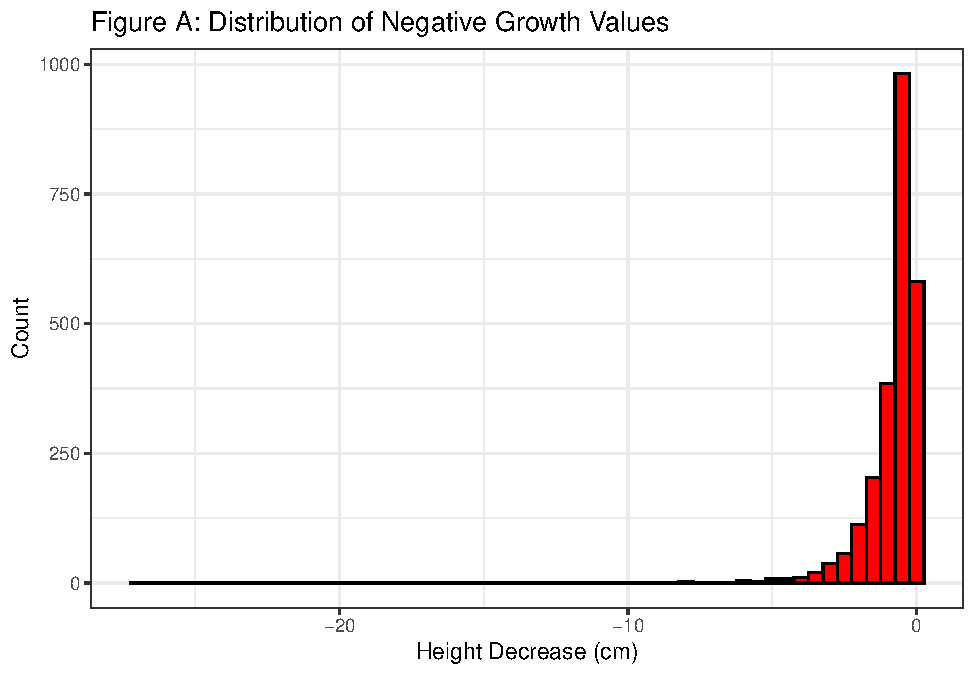
\includegraphics[keepaspectratio]{WK8_files/figure-latex/unnamed-chunk-4-1.pdf}}

\begin{Shaded}
\begin{Highlighting}[]
\CommentTok{\#filter out plants with negative growth \textless{} {-}5}
\NormalTok{plant\_growth\_cleaned }\OtherTok{\textless{}{-}}\NormalTok{ plant\_growth}

\ControlFlowTok{repeat}\NormalTok{ \{}
\NormalTok{  plant\_growth\_cleaned }\OtherTok{\textless{}{-}}\NormalTok{ plant\_growth\_cleaned }\SpecialCharTok{\%\textgreater{}\%}
    \FunctionTok{arrange}\NormalTok{(PID, survey\_date) }\SpecialCharTok{\%\textgreater{}\%}
    \FunctionTok{group\_by}\NormalTok{(PID) }\SpecialCharTok{\%\textgreater{}\%}
    \FunctionTok{mutate}\NormalTok{(}\AttributeTok{growth =}\NormalTok{ height\_cm }\SpecialCharTok{{-}} \FunctionTok{lag}\NormalTok{(height\_cm)) }\SpecialCharTok{\%\textgreater{}\%}
    \FunctionTok{filter}\NormalTok{(}\FunctionTok{is.na}\NormalTok{(growth) }\SpecialCharTok{|}\NormalTok{ growth }\SpecialCharTok{\textgreater{}=} \SpecialCharTok{{-}}\DecValTok{5}\NormalTok{) }\SpecialCharTok{\%\textgreater{}\%}
    \FunctionTok{select}\NormalTok{(}\SpecialCharTok{{-}}\NormalTok{growth) }\SpecialCharTok{\%\textgreater{}\%}
    \FunctionTok{ungroup}\NormalTok{()}

\NormalTok{  check }\OtherTok{\textless{}{-}}\NormalTok{ plant\_growth\_cleaned }\SpecialCharTok{\%\textgreater{}\%}
    \FunctionTok{arrange}\NormalTok{(PID, survey\_date) }\SpecialCharTok{\%\textgreater{}\%}
    \FunctionTok{group\_by}\NormalTok{(PID) }\SpecialCharTok{\%\textgreater{}\%}
    \FunctionTok{mutate}\NormalTok{(}\AttributeTok{growth =}\NormalTok{ height\_cm }\SpecialCharTok{{-}} \FunctionTok{lag}\NormalTok{(height\_cm)) }\SpecialCharTok{\%\textgreater{}\%}
    \FunctionTok{filter}\NormalTok{(growth }\SpecialCharTok{\textless{}} \SpecialCharTok{{-}}\DecValTok{5}\NormalTok{)}
  
  \ControlFlowTok{if}\NormalTok{ (}\FunctionTok{nrow}\NormalTok{(check) }\SpecialCharTok{==} \DecValTok{0}\NormalTok{) }\ControlFlowTok{break}
\NormalTok{\}}
\end{Highlighting}
\end{Shaded}

\emph{Measure Growth via Daily Growth Rate}

\begin{Shaded}
\begin{Highlighting}[]
\CommentTok{\#define daily growth rate}
\NormalTok{plant\_growth\_daily }\OtherTok{\textless{}{-}}\NormalTok{ plant\_growth\_cleaned }\SpecialCharTok{\%\textgreater{}\%}
  \FunctionTok{arrange}\NormalTok{(PID, survey\_date) }\SpecialCharTok{\%\textgreater{}\%}
  \FunctionTok{group\_by}\NormalTok{(PID) }\SpecialCharTok{\%\textgreater{}\%}
  \FunctionTok{mutate}\NormalTok{(}
    \AttributeTok{prev\_height =} \FunctionTok{lag}\NormalTok{(height\_cm),}
    \AttributeTok{prev\_date =} \FunctionTok{lag}\NormalTok{(survey\_date),}
    \AttributeTok{days\_elapsed =} \FunctionTok{as.numeric}\NormalTok{(survey\_date }\SpecialCharTok{{-}}\NormalTok{ prev\_date),}
    \AttributeTok{daily\_growth =}\NormalTok{ (height\_cm }\SpecialCharTok{{-}}\NormalTok{ prev\_height) }\SpecialCharTok{/}\NormalTok{ days\_elapsed}
\NormalTok{  ) }\SpecialCharTok{\%\textgreater{}\%}
  \FunctionTok{ungroup}\NormalTok{()}
\end{Highlighting}
\end{Shaded}

\emph{Correlate Growth with Solar Radiation} \#Q: How does plant growth
correlate with solar radiation? \#Test: Find correlation value and plot
correlation \#Figure B: Scatter plot showing the relationship between
weekly average solar radiation (SlrW, W/m²) and daily growth rate
(cm/day). Each point represents an observation, and the red line
indicates the fitted linear regression.

\begin{Shaded}
\begin{Highlighting}[]
\CommentTok{\#Align plant growth data to week}
\NormalTok{plant\_weekly }\OtherTok{\textless{}{-}}\NormalTok{ plant\_growth\_daily }\SpecialCharTok{\%\textgreater{}\%}
  \FunctionTok{filter}\NormalTok{(}\SpecialCharTok{!}\FunctionTok{is.na}\NormalTok{(daily\_growth), days\_elapsed }\SpecialCharTok{\textgreater{}} \DecValTok{0}\NormalTok{) }\SpecialCharTok{\%\textgreater{}\%}
  \FunctionTok{mutate}\NormalTok{(}\AttributeTok{week =} \FunctionTok{floor\_date}\NormalTok{(survey\_date, }\StringTok{"week"}\NormalTok{))}

\CommentTok{\#Adds \textasciigrave{}weekly\_avg\_SlrW\textasciigrave{} to plant data}
\NormalTok{plant\_with\_light }\OtherTok{\textless{}{-}}\NormalTok{ plant\_weekly }\SpecialCharTok{\%\textgreater{}\%}
  \FunctionTok{left\_join}\NormalTok{(weekly\_light, }\AttributeTok{by =} \StringTok{"week"}\NormalTok{)}

\CommentTok{\#Calculate correlation}
\NormalTok{cor\_result }\OtherTok{\textless{}{-}} \FunctionTok{cor}\NormalTok{(}
\NormalTok{  plant\_with\_light}\SpecialCharTok{$}\NormalTok{daily\_growth,}
\NormalTok{  plant\_with\_light}\SpecialCharTok{$}\NormalTok{weekly\_avg\_SlrW,}
\AttributeTok{use =} \StringTok{"complete.obs"}
\NormalTok{)}

\FunctionTok{print}\NormalTok{(cor\_result)}
\end{Highlighting}
\end{Shaded}

\begin{verbatim}
## [1] 0.1299395
\end{verbatim}

\begin{Shaded}
\begin{Highlighting}[]
\CommentTok{\#Plot correlation}
\FunctionTok{ggplot}\NormalTok{(plant\_with\_light, }\FunctionTok{aes}\NormalTok{(}\AttributeTok{x =}\NormalTok{ weekly\_avg\_SlrW, }\AttributeTok{y =}\NormalTok{ daily\_growth)) }\SpecialCharTok{+}
  \FunctionTok{geom\_point}\NormalTok{(}\AttributeTok{alpha =} \FloatTok{0.2}\NormalTok{) }\SpecialCharTok{+}
  \FunctionTok{geom\_smooth}\NormalTok{(}\AttributeTok{method =} \StringTok{"lm"}\NormalTok{, }\AttributeTok{color =} \StringTok{"red"}\NormalTok{) }\SpecialCharTok{+}
  \FunctionTok{labs}\NormalTok{(}\AttributeTok{title =} \StringTok{"Figure B: Correlation between Light and Growth"}\NormalTok{, }\AttributeTok{x =} \StringTok{"Weekly Avg Light (SlrW)"}\NormalTok{, }\AttributeTok{y =} \StringTok{"Daily Growth (cm/day)"}\NormalTok{) }\SpecialCharTok{+}
  \FunctionTok{theme\_bw}\NormalTok{()}
\end{Highlighting}
\end{Shaded}

\begin{verbatim}
## `geom_smooth()` using formula = 'y ~ x'
\end{verbatim}

\begin{verbatim}
## Warning: Removed 1069 rows containing non-finite outside the scale range
## (`stat_smooth()`).
\end{verbatim}

\begin{verbatim}
## Warning: Removed 1069 rows containing missing values or values outside the scale range
## (`geom_point()`).
\end{verbatim}

\pandocbounded{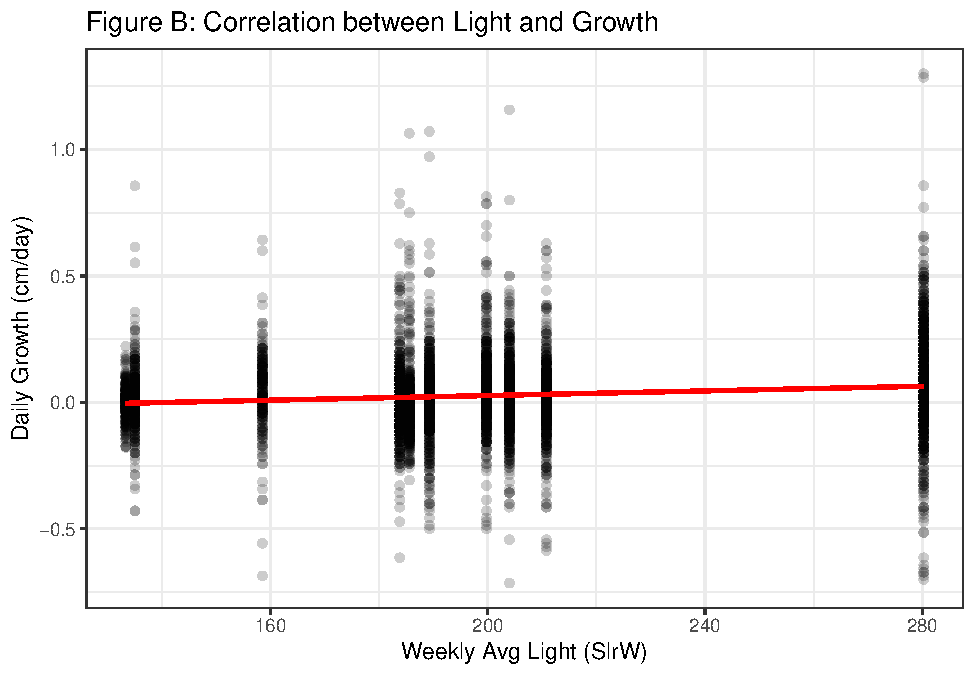
\includegraphics[keepaspectratio]{WK8_files/figure-latex/unnamed-chunk-6-1.pdf}}

\emph{Process data}

\begin{Shaded}
\begin{Highlighting}[]
\CommentTok{\#Standardization}
\NormalTok{plant\_with\_light}\SpecialCharTok{$}\NormalTok{weekly\_avg\_SlrW2 }\OtherTok{\textless{}{-}} \FunctionTok{scale}\NormalTok{(plant\_with\_light}\SpecialCharTok{$}\NormalTok{weekly\_avg\_SlrW, }\AttributeTok{center =} \ConstantTok{TRUE}\NormalTok{, }\AttributeTok{scale =} \ConstantTok{TRUE}\NormalTok{)}
\NormalTok{mean\_light }\OtherTok{\textless{}{-}} \FunctionTok{mean}\NormalTok{(plant\_with\_light}\SpecialCharTok{$}\NormalTok{weekly\_avg\_SlrW, }\AttributeTok{na.rm =} \ConstantTok{TRUE}\NormalTok{)}
\NormalTok{sd\_light   }\OtherTok{\textless{}{-}} \FunctionTok{sd}\NormalTok{(plant\_with\_light}\SpecialCharTok{$}\NormalTok{weekly\_avg\_SlrW, }\AttributeTok{na.rm =} \ConstantTok{TRUE}\NormalTok{)}

\CommentTok{\#Change Data type}
\NormalTok{plant\_with\_light }\OtherTok{\textless{}{-}}\NormalTok{ plant\_with\_light }\SpecialCharTok{\%\textgreater{}\%}
  \FunctionTok{mutate}\NormalTok{(}
    \AttributeTok{parent\_pop =} \FunctionTok{factor}\NormalTok{(parent\_pop),}
    \AttributeTok{PID        =} \FunctionTok{factor}\NormalTok{(PID),}
    \AttributeTok{block      =} \FunctionTok{factor}\NormalTok{(block)}
\NormalTok{  )}
\end{Highlighting}
\end{Shaded}

\emph{use mixed-effect model to fit relationship between plant growth
and light radiation with population as random effect} \#Q: Does weekly
solar radiation positively affect daily growth rate across all
populations? \#Test: Fit a mixed-effect model with population as a
random slope.

\begin{Shaded}
\begin{Highlighting}[]
\NormalTok{growth\_light.lmer }\OtherTok{\textless{}{-}} \FunctionTok{lmer}\NormalTok{(}
\NormalTok{  daily\_growth }\SpecialCharTok{\textasciitilde{}}\NormalTok{ weekly\_avg\_SlrW2 }\SpecialCharTok{+}                     
\NormalTok{    (}\DecValTok{1} \SpecialCharTok{+}\NormalTok{ weekly\_avg\_SlrW2 }\SpecialCharTok{|}\NormalTok{ parent\_pop),                                    }
  \AttributeTok{data =}\NormalTok{ plant\_with\_light, }\AttributeTok{REML =} \ConstantTok{TRUE}
\NormalTok{)}
\FunctionTok{summary}\NormalTok{(growth\_light.lmer)}
\end{Highlighting}
\end{Shaded}

\begin{verbatim}
## Linear mixed model fit by REML ['lmerMod']
## Formula: daily_growth ~ weekly_avg_SlrW2 + (1 + weekly_avg_SlrW2 | parent_pop)
##    Data: plant_with_light
## 
## REML criterion at convergence: -6464.1
## 
## Scaled residuals: 
##     Min      1Q  Median      3Q     Max 
## -6.2096 -0.4715  0.0094  0.4415  8.3380 
## 
## Random effects:
##  Groups     Name             Variance  Std.Dev. Corr
##  parent_pop (Intercept)      0.0015837 0.0398       
##             weekly_avg_SlrW2 0.0002495 0.0158   0.03
##  Residual                    0.0191023 0.1382       
## Number of obs: 5870, groups:  parent_pop, 22
## 
## Fixed effects:
##                  Estimate Std. Error t value
## (Intercept)      0.017235   0.008784   1.962
## weekly_avg_SlrW2 0.024127   0.003973   6.073
## 
## Correlation of Fixed Effects:
##             (Intr)
## wkly_vg_SW2 0.020
\end{verbatim}

\emph{overall effect of solar radiation on plant daily growth} \#Figure
C: Relationship between weekly average solar radiation and predicted
daily growth rate (cm/day), aggregated across all populations. Each
hexagon represents the density of observations. The black line shows the
fitted regression slope .

\begin{Shaded}
\begin{Highlighting}[]
\CommentTok{\#Unscaling}
\NormalTok{pred\_all }\OtherTok{\textless{}{-}} \FunctionTok{ggpredict}\NormalTok{(growth\_light.lmer, }\AttributeTok{terms =} \StringTok{"weekly\_avg\_SlrW2"}\NormalTok{) }\SpecialCharTok{\%\textgreater{}\%}
  \FunctionTok{as.data.frame}\NormalTok{() }\SpecialCharTok{\%\textgreater{}\%}
  \FunctionTok{mutate}\NormalTok{(}\AttributeTok{light\_orig =}\NormalTok{ x }\SpecialCharTok{*}\NormalTok{ sd\_light }\SpecialCharTok{+}\NormalTok{ mean\_light)}

\CommentTok{\#Plot}
\NormalTok{p\_overall }\OtherTok{\textless{}{-}} \FunctionTok{ggplot}\NormalTok{() }\SpecialCharTok{+}
  \FunctionTok{geom\_hex}\NormalTok{(}\AttributeTok{data =}\NormalTok{ plant\_with\_light,}
           \FunctionTok{aes}\NormalTok{(}\AttributeTok{x =}\NormalTok{ weekly\_avg\_SlrW, }\AttributeTok{y =}\NormalTok{ daily\_growth), }\AttributeTok{bins =} \DecValTok{35}\NormalTok{) }\SpecialCharTok{+}
  \FunctionTok{scale\_fill\_viridis\_c}\NormalTok{(}\AttributeTok{name =} \StringTok{"Count"}\NormalTok{) }\SpecialCharTok{+}
  \FunctionTok{geom\_ribbon}\NormalTok{(}\AttributeTok{data =}\NormalTok{ pred\_all,}
              \FunctionTok{aes}\NormalTok{(}\AttributeTok{x =}\NormalTok{ light\_orig, }\AttributeTok{ymin =}\NormalTok{ conf.low, }\AttributeTok{ymax =}\NormalTok{ conf.high),}
              \AttributeTok{alpha =}\NormalTok{ .}\DecValTok{22}\NormalTok{, }\AttributeTok{fill =} \StringTok{"grey60"}\NormalTok{) }\SpecialCharTok{+}
  \FunctionTok{geom\_line}\NormalTok{(}\AttributeTok{data =}\NormalTok{ pred\_all,}
            \FunctionTok{aes}\NormalTok{(}\AttributeTok{x =}\NormalTok{ light\_orig, }\AttributeTok{y =}\NormalTok{ predicted), }\AttributeTok{linewidth =} \DecValTok{1}\NormalTok{) }\SpecialCharTok{+}
  \FunctionTok{labs}\NormalTok{(}\AttributeTok{title =} \StringTok{"Figure C: Effect of Weekly Light on Daily Growth (overall)"}\NormalTok{,}
       \AttributeTok{x =} \StringTok{"Weekly Avg Light (W/m²)"}\NormalTok{,}
       \AttributeTok{y =} \StringTok{"Predicted Daily Growth (cm/day)"}\NormalTok{) }\SpecialCharTok{+}
  \FunctionTok{theme\_bw}\NormalTok{() }\SpecialCharTok{+}
  \FunctionTok{theme}\NormalTok{(}\AttributeTok{panel.grid.minor =} \FunctionTok{element\_blank}\NormalTok{())}
\NormalTok{p\_overall}
\end{Highlighting}
\end{Shaded}

\begin{verbatim}
## Warning: Removed 1069 rows containing non-finite outside the scale range
## (`stat_binhex()`).
\end{verbatim}

\pandocbounded{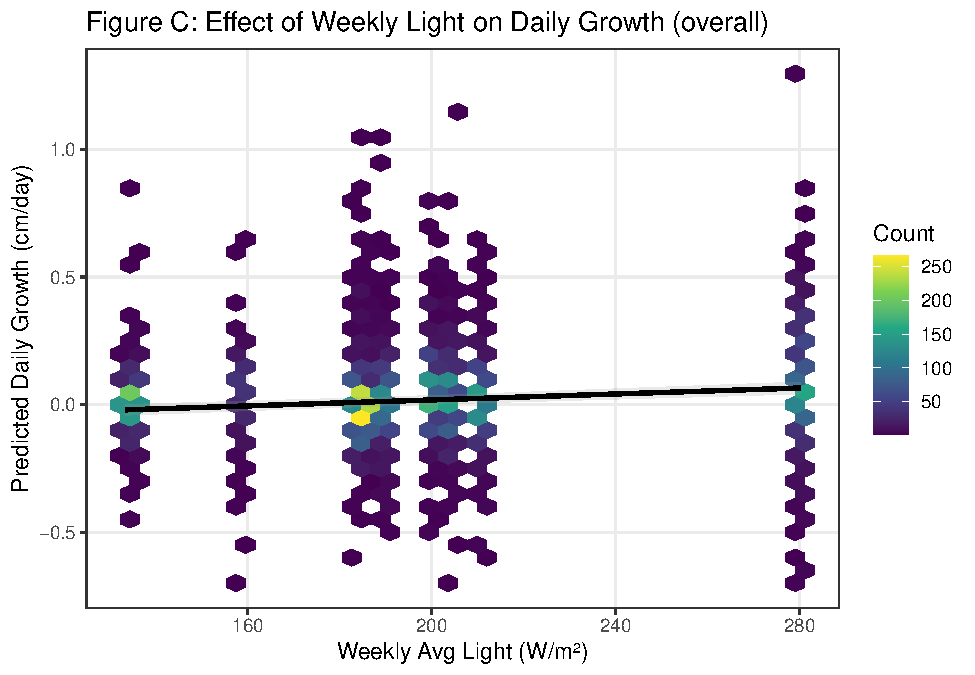
\includegraphics[keepaspectratio]{WK8_files/figure-latex/unnamed-chunk-9-1.pdf}}

\emph{Effect of solar radiation on plant daily growth by population}
\#Q: Do different populations vary in their growth response to weekly
solar radiation? \#Test: For visualization, scatter plots with fitted
regression lines were drawn separately for each population. \#Figure D:
Light--growth relationship by population. \#Scatter plots show daily
growth rate (cm/day) against weekly average solar radiation (W/m²) for
22 populations. Each panel corresponds to one population, with the blue
line indicating the fitted linear trend.

\begin{Shaded}
\begin{Highlighting}[]
\NormalTok{p\_facet }\OtherTok{\textless{}{-}} \FunctionTok{ggplot}\NormalTok{(plant\_with\_light,}
                  \FunctionTok{aes}\NormalTok{(weekly\_avg\_SlrW, daily\_growth)) }\SpecialCharTok{+}
  \FunctionTok{facet\_wrap}\NormalTok{(}\SpecialCharTok{\textasciitilde{}}\NormalTok{ parent\_pop, }\AttributeTok{ncol =} \DecValTok{6}\NormalTok{) }\SpecialCharTok{+}
  \FunctionTok{geom\_point}\NormalTok{(}\AttributeTok{alpha =}\NormalTok{ .}\DecValTok{15}\NormalTok{, }\AttributeTok{size =}\NormalTok{ .}\DecValTok{6}\NormalTok{, }\AttributeTok{color =} \StringTok{"grey35"}\NormalTok{) }\SpecialCharTok{+}
  \FunctionTok{geom\_smooth}\NormalTok{(}\AttributeTok{method =} \StringTok{"lm"}\NormalTok{, }\AttributeTok{se =} \ConstantTok{FALSE}\NormalTok{, }\AttributeTok{linewidth =}\NormalTok{ .}\DecValTok{8}\NormalTok{) }\SpecialCharTok{+}
  \FunctionTok{labs}\NormalTok{(}\AttributeTok{title =} \StringTok{"Figure D: Light–Growth relationship by population"}\NormalTok{,}
       \AttributeTok{x =} \StringTok{"Weekly Avg Light (W/m²)"}\NormalTok{,}
       \AttributeTok{y =} \StringTok{"Daily Growth (cm/day)"}\NormalTok{) }\SpecialCharTok{+}
  \FunctionTok{theme\_bw}\NormalTok{() }\SpecialCharTok{+}
  \FunctionTok{theme}\NormalTok{(}\AttributeTok{strip.background =} \FunctionTok{element\_rect}\NormalTok{(}\AttributeTok{fill =} \StringTok{"grey95"}\NormalTok{, }\AttributeTok{color =} \ConstantTok{NA}\NormalTok{),}
        \AttributeTok{strip.text =} \FunctionTok{element\_text}\NormalTok{(}\AttributeTok{face =} \StringTok{"bold"}\NormalTok{),}
        \AttributeTok{panel.grid.minor =} \FunctionTok{element\_blank}\NormalTok{())}
\NormalTok{p\_facet}
\end{Highlighting}
\end{Shaded}

\begin{verbatim}
## `geom_smooth()` using formula = 'y ~ x'
\end{verbatim}

\begin{verbatim}
## Warning: Removed 1069 rows containing non-finite outside the scale range
## (`stat_smooth()`).
\end{verbatim}

\begin{verbatim}
## Warning: Removed 1069 rows containing missing values or values outside the scale range
## (`geom_point()`).
\end{verbatim}

\pandocbounded{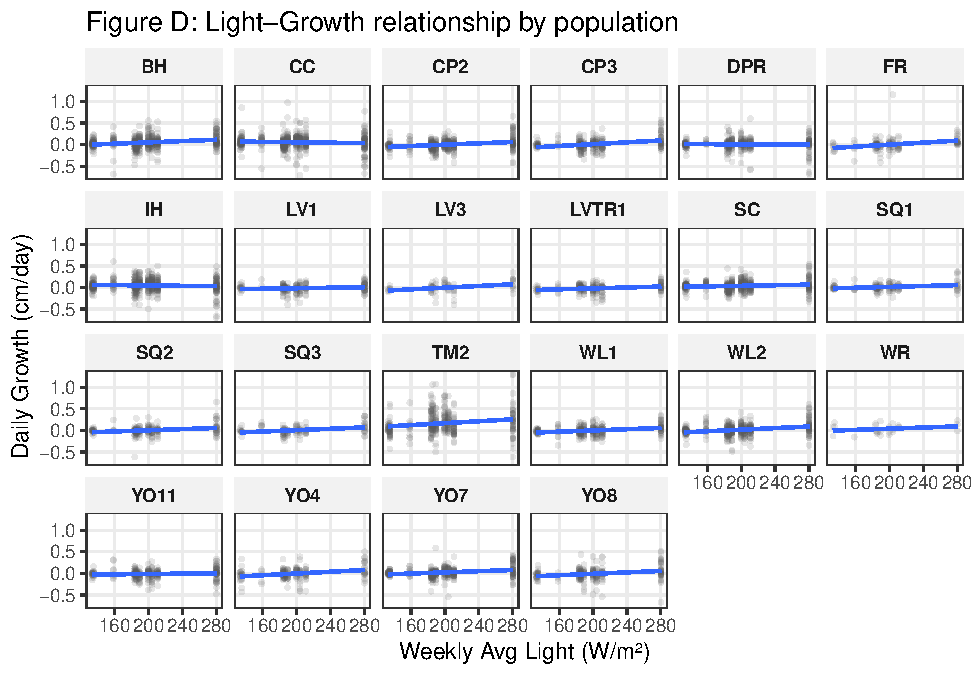
\includegraphics[keepaspectratio]{WK8_files/figure-latex/unnamed-chunk-10-1.pdf}}

\emph{Find slope of plant growth and solar radiation for each
population} \#Q: Which populations show significantly positive or
negligible slopes in the light--growth relationship? \#Method: Extract
slopes and 95\% confidence intervals for each population from the
mixed-effects model \#Figure E. Population-specific slopes with 95\%
confidence intervals. \#Forest plot showing estimated slopes of daily
growth rate against weekly average solar radiation for 22 populations.
Points represent population-specific slopes (cm/day per W/m²) and
horizontal lines show 95\% CIs. Several populations (e.g., TM2, CP3, FR,
WL2, YO4) exhibit significantly positive slopes with CIs entirely above
zero, indicating stronger growth response to light. Others (e.g., CC,
IH, DPR) have slopes not significantly different from zero, suggesting
little or no detectable response to light.

\begin{Shaded}
\begin{Highlighting}[]
\CommentTok{\#slope and standard deviation of fixed effects}
\NormalTok{b\_fix  }\OtherTok{\textless{}{-}} \FunctionTok{fixef}\NormalTok{(growth\_light.lmer)[}\StringTok{"weekly\_avg\_SlrW2"}\NormalTok{]}
\NormalTok{V\_fix  }\OtherTok{\textless{}{-}} \FunctionTok{vcov}\NormalTok{(growth\_light.lmer)[}\StringTok{"weekly\_avg\_SlrW2"}\NormalTok{,}\StringTok{"weekly\_avg\_SlrW2"}\NormalTok{]}

\CommentTok{\#slope and standard deviation of random effects}
\NormalTok{re }\OtherTok{\textless{}{-}} \FunctionTok{ranef}\NormalTok{(growth\_light.lmer, }\AttributeTok{condVar =} \ConstantTok{TRUE}\NormalTok{) }
\NormalTok{re\_pop }\OtherTok{\textless{}{-}}\NormalTok{ re}\SpecialCharTok{$}\NormalTok{parent\_pop}
\NormalTok{postVar }\OtherTok{\textless{}{-}} \FunctionTok{attr}\NormalTok{(re}\SpecialCharTok{$}\NormalTok{parent\_pop, }\StringTok{"postVar"}\NormalTok{)           }
\NormalTok{sl\_col }\OtherTok{\textless{}{-}} \FunctionTok{which}\NormalTok{(}\FunctionTok{colnames}\NormalTok{(re\_pop) }\SpecialCharTok{==} \StringTok{"weekly\_avg\_SlrW2"}\NormalTok{)}

\CommentTok{\#create the tibble of slopes for each population}
\NormalTok{pop\_slope }\OtherTok{\textless{}{-}} \FunctionTok{tibble}\NormalTok{(}
  \AttributeTok{parent\_pop   =} \FunctionTok{rownames}\NormalTok{(re\_pop),}
  \AttributeTok{rand\_slope   =}\NormalTok{ re\_pop[ , }\StringTok{"weekly\_avg\_SlrW2"}\NormalTok{],}
  \AttributeTok{rand\_var     =} \FunctionTok{sapply}\NormalTok{(}\FunctionTok{seq\_len}\NormalTok{(}\FunctionTok{dim}\NormalTok{(postVar)[}\DecValTok{3}\NormalTok{]), }\ControlFlowTok{function}\NormalTok{(i) postVar[sl\_col, sl\_col, i])}
\NormalTok{) }\SpecialCharTok{\%\textgreater{}\%}
  \FunctionTok{mutate}\NormalTok{(}
    \AttributeTok{slope\_SD   =}\NormalTok{ b\_fix }\SpecialCharTok{+}\NormalTok{ rand\_slope,                        }
    \AttributeTok{se\_SD      =} \FunctionTok{sqrt}\NormalTok{(V\_fix }\SpecialCharTok{+}\NormalTok{ rand\_var),               }
    \AttributeTok{lower\_SD   =}\NormalTok{ slope\_SD }\SpecialCharTok{{-}} \FloatTok{1.96}\SpecialCharTok{*}\NormalTok{se\_SD,}
    \AttributeTok{upper\_SD   =}\NormalTok{ slope\_SD }\SpecialCharTok{+} \FloatTok{1.96}\SpecialCharTok{*}\NormalTok{se\_SD}
\NormalTok{  )}

\NormalTok{sd\_light }\OtherTok{\textless{}{-}} \FunctionTok{sd}\NormalTok{(plant\_with\_light}\SpecialCharTok{$}\NormalTok{weekly\_avg\_SlrW, }\AttributeTok{na.rm =} \ConstantTok{TRUE}\NormalTok{)}

\NormalTok{pop\_slope }\OtherTok{\textless{}{-}}\NormalTok{ pop\_slope }\SpecialCharTok{\%\textgreater{}\%}
  \FunctionTok{mutate}\NormalTok{(}
    \AttributeTok{slope\_per\_Wm2 =}\NormalTok{ slope\_SD }\SpecialCharTok{/}\NormalTok{ sd\_light,}
    \AttributeTok{lower\_per\_Wm2 =}\NormalTok{ lower\_SD }\SpecialCharTok{/}\NormalTok{ sd\_light,}
    \AttributeTok{upper\_per\_Wm2 =}\NormalTok{ upper\_SD }\SpecialCharTok{/}\NormalTok{ sd\_light}
\NormalTok{  )}\SpecialCharTok{\%\textgreater{}\%}
  \FunctionTok{select}\NormalTok{(parent\_pop, slope\_per\_Wm2, lower\_per\_Wm2, upper\_per\_Wm2)}
\NormalTok{pop\_slope}
\end{Highlighting}
\end{Shaded}

\begin{verbatim}
## # A tibble: 22 x 4
##    parent_pop slope_per_Wm2 lower_per_Wm2 upper_per_Wm2
##    <chr>              <dbl>         <dbl>         <dbl>
##  1 BH             0.000742      0.000409       0.00108 
##  2 CC            -0.000128     -0.000461       0.000205
##  3 CP2            0.000744      0.000376       0.00111 
##  4 CP3            0.000949      0.000542       0.00136 
##  5 DPR            0.0000489    -0.000316       0.000413
##  6 FR             0.000918      0.000402       0.00143 
##  7 IH            -0.000105     -0.000433       0.000223
##  8 LV1            0.000373     -0.0000792      0.000825
##  9 LV3            0.000755      0.000174       0.00134 
## 10 LVTR1          0.000540      0.0000734      0.00101 
## # i 12 more rows
\end{verbatim}

\begin{Shaded}
\begin{Highlighting}[]
\FunctionTok{write.csv}\NormalTok{(pop\_slope, }\StringTok{"population\_slopes.csv"}\NormalTok{, }\AttributeTok{row.names =} \ConstantTok{FALSE}\NormalTok{)}

\CommentTok{\#plot}
\FunctionTok{ggplot}\NormalTok{(pop\_slope, }\FunctionTok{aes}\NormalTok{(}\AttributeTok{x =} \FunctionTok{reorder}\NormalTok{(parent\_pop, slope\_per\_Wm2), }\AttributeTok{y =}\NormalTok{ slope\_per\_Wm2)) }\SpecialCharTok{+}
  \FunctionTok{geom\_hline}\NormalTok{(}\AttributeTok{yintercept =} \DecValTok{0}\NormalTok{, }\AttributeTok{linetype =} \DecValTok{2}\NormalTok{) }\SpecialCharTok{+}
  \FunctionTok{geom\_pointrange}\NormalTok{(}\FunctionTok{aes}\NormalTok{(}\AttributeTok{ymin =}\NormalTok{ lower\_per\_Wm2, }\AttributeTok{ymax =}\NormalTok{ upper\_per\_Wm2), }\AttributeTok{linewidth =}\NormalTok{ .}\DecValTok{6}\NormalTok{) }\SpecialCharTok{+}
  \FunctionTok{coord\_flip}\NormalTok{() }\SpecialCharTok{+}
  \FunctionTok{labs}\NormalTok{(}\AttributeTok{title =} \StringTok{"Figure E: Population{-}specific slopes with 95\% CI"}\NormalTok{,}
       \AttributeTok{x =} \StringTok{"Population"}\NormalTok{, }\AttributeTok{y =} \StringTok{"Slope (cm/day per W/m²)"}\NormalTok{) }\SpecialCharTok{+}
  \FunctionTok{theme\_bw}\NormalTok{()}
\end{Highlighting}
\end{Shaded}

\pandocbounded{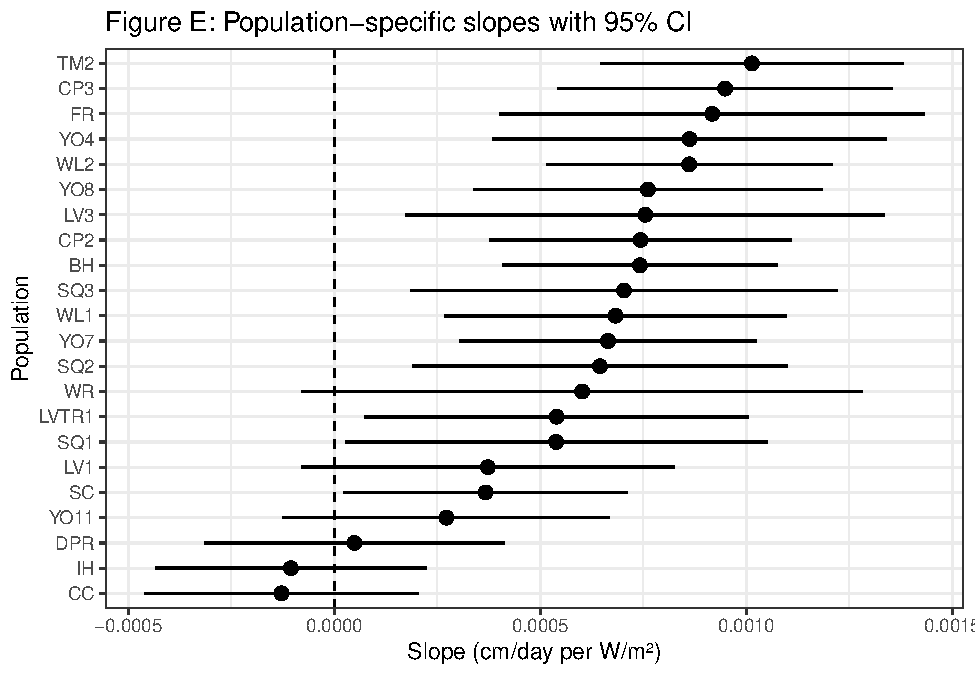
\includegraphics[keepaspectratio]{WK8_files/figure-latex/unnamed-chunk-11-1.pdf}}

\emph{height\_time plot with solar radiation as color}

\begin{Shaded}
\begin{Highlighting}[]
\NormalTok{light\_daily }\OtherTok{\textless{}{-}}\NormalTok{ light\_raw }\SpecialCharTok{\%\textgreater{}\%}
  \FunctionTok{mutate}\NormalTok{(}\AttributeTok{date =} \FunctionTok{as.Date}\NormalTok{(TIMESTAMP)) }\SpecialCharTok{\%\textgreater{}\%}
  \FunctionTok{group\_by}\NormalTok{(date) }\SpecialCharTok{\%\textgreater{}\%}
  \FunctionTok{summarise}\NormalTok{(}\AttributeTok{SlrW\_mean =} \FunctionTok{mean}\NormalTok{(SlrW\_Avg, }\AttributeTok{na.rm =} \ConstantTok{TRUE}\NormalTok{), }\AttributeTok{.groups =} \StringTok{"drop"}\NormalTok{)}

\NormalTok{df\_plot }\OtherTok{\textless{}{-}}\NormalTok{ plant\_with\_light }\SpecialCharTok{\%\textgreater{}\%}
  \FunctionTok{filter}\NormalTok{(}\SpecialCharTok{!}\FunctionTok{is.na}\NormalTok{(survey\_date), }\SpecialCharTok{!}\FunctionTok{is.na}\NormalTok{(height\_cm), }\SpecialCharTok{!}\FunctionTok{is.na}\NormalTok{(weekly\_avg\_SlrW))}

\NormalTok{y\_rng     }\OtherTok{\textless{}{-}} \FunctionTok{range}\NormalTok{(df\_plot}\SpecialCharTok{$}\NormalTok{height\_cm, }\AttributeTok{na.rm =} \ConstantTok{TRUE}\NormalTok{)}
\NormalTok{light\_rng }\OtherTok{\textless{}{-}} \FunctionTok{range}\NormalTok{(light\_daily}\SpecialCharTok{$}\NormalTok{SlrW\_mean, }\AttributeTok{na.rm =} \ConstantTok{TRUE}\NormalTok{)}

\NormalTok{light\_daily }\OtherTok{\textless{}{-}}\NormalTok{ light\_daily }\SpecialCharTok{\%\textgreater{}\%}
  \FunctionTok{mutate}\NormalTok{(}\AttributeTok{light\_y =}\NormalTok{ scales}\SpecialCharTok{::}\FunctionTok{rescale}\NormalTok{(SlrW\_mean, }\AttributeTok{to =}\NormalTok{ y\_rng, }\AttributeTok{from =}\NormalTok{ light\_rng))}

\NormalTok{plant\_with\_light}\SpecialCharTok{\%\textgreater{}\%}
  \FunctionTok{group\_by}\NormalTok{(parent\_pop)}\SpecialCharTok{\%\textgreater{}\%}
  \FunctionTok{ggplot}\NormalTok{(}\FunctionTok{aes}\NormalTok{(survey\_date, height\_cm, }\AttributeTok{colour =}\NormalTok{ weekly\_avg\_SlrW)) }\SpecialCharTok{+}
  \FunctionTok{geom\_line}\NormalTok{(}\AttributeTok{data =}\NormalTok{ light\_daily,}
            \FunctionTok{aes}\NormalTok{(}\AttributeTok{x =}\NormalTok{ date, }\AttributeTok{y =}\NormalTok{ light\_y),}
            \AttributeTok{colour =} \StringTok{"black"}\NormalTok{, }\AttributeTok{linewidth =} \FloatTok{0.5}\NormalTok{, }\AttributeTok{alpha=} \FloatTok{0.25}\NormalTok{) }\SpecialCharTok{+}
  \FunctionTok{facet\_wrap}\NormalTok{(}\SpecialCharTok{\textasciitilde{}}\NormalTok{parent\_pop)}\SpecialCharTok{+}
  \FunctionTok{scale\_colour\_gradientn}\NormalTok{(                         }\CommentTok{\# 低=蓝,高=红}
    \AttributeTok{colours =} \FunctionTok{c}\NormalTok{(}\StringTok{"\#2c7bb6"}\NormalTok{,}\StringTok{"\#abd9e9"}\NormalTok{,}\StringTok{"\#ffffbf"}\NormalTok{,}\StringTok{"\#fdae61"}\NormalTok{,}\StringTok{"\#d7191c"}\NormalTok{),}
    \AttributeTok{name =} \StringTok{"solar radiation (W/m²)"}\NormalTok{)}\SpecialCharTok{+}
  \FunctionTok{geom\_point}\NormalTok{(}\AttributeTok{alpha=}\FloatTok{0.25}\NormalTok{,}\AttributeTok{size=}\FloatTok{0.5}\NormalTok{)}\SpecialCharTok{+}
  \FunctionTok{geom\_line}\NormalTok{(}\AttributeTok{alpha=}\DecValTok{1}\NormalTok{, }\AttributeTok{size=}\DecValTok{1}\NormalTok{) }\SpecialCharTok{+}
  \FunctionTok{scale\_x\_date}\NormalTok{(}\AttributeTok{date\_breaks =} \StringTok{"1 month"}\NormalTok{, }\AttributeTok{date\_labels =} \StringTok{"\%b"}\NormalTok{) }\SpecialCharTok{+}
   \FunctionTok{scale\_y\_continuous}\NormalTok{(}
    \AttributeTok{name =} \StringTok{"Height (cm)"}\NormalTok{,}
    \AttributeTok{sec.axis =} \FunctionTok{sec\_axis}\NormalTok{(}\SpecialCharTok{\textasciitilde{}}\NormalTok{ scales}\SpecialCharTok{::}\FunctionTok{rescale}\NormalTok{(., }\AttributeTok{from =}\NormalTok{ y\_rng, }\AttributeTok{to =}\NormalTok{ light\_rng),}
                        \AttributeTok{name =} \StringTok{"Solar Radiation (W/m²)"}\NormalTok{))}\SpecialCharTok{+}
  \FunctionTok{labs}\NormalTok{(}\AttributeTok{title =} \StringTok{"Figure F: Time{-}Height"}\NormalTok{,}
       \AttributeTok{x =} \StringTok{"Survey Date"}\NormalTok{,}
       \AttributeTok{y =} \StringTok{"Height (cm)"}\NormalTok{) }\SpecialCharTok{+}
  \FunctionTok{theme\_bw}\NormalTok{()}
\end{Highlighting}
\end{Shaded}

\begin{verbatim}
## Warning: Using `size` aesthetic for lines was deprecated in ggplot2 3.4.0.
## i Please use `linewidth` instead.
## This warning is displayed once every 8 hours.
## Call `lifecycle::last_lifecycle_warnings()` to see where this warning was
## generated.
\end{verbatim}

\pandocbounded{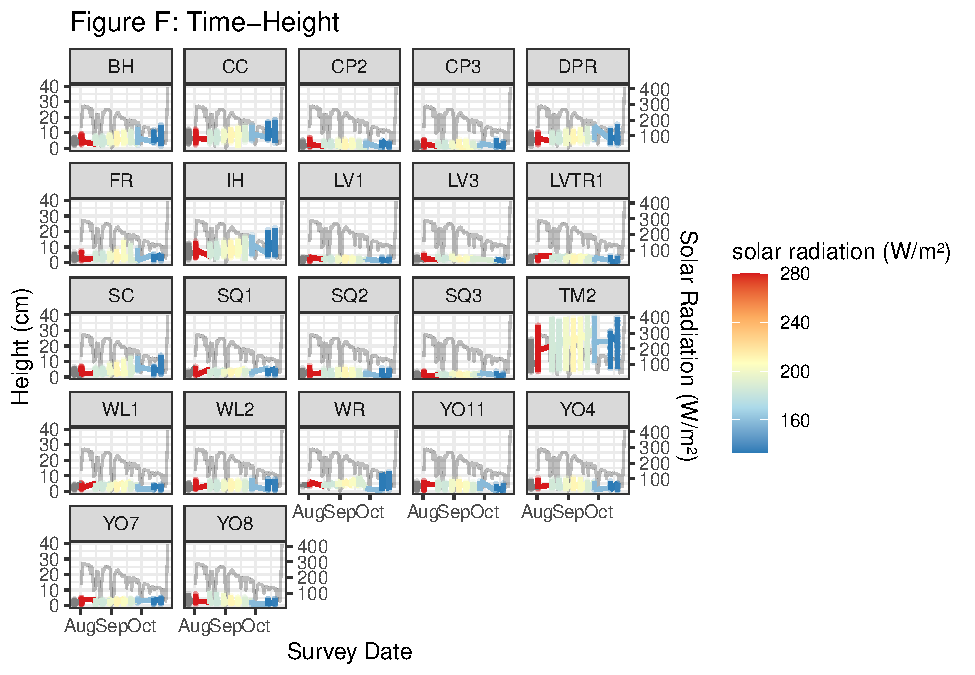
\includegraphics[keepaspectratio]{WK8_files/figure-latex/unnamed-chunk-12-1.pdf}}

\end{document}
